\definecolor{new_red}{rgb}{0.95,0.47,0.47}
\definecolor{new_green}{rgb}{0.85,0.98,0.77}

\begin{figure}[!htb]
\vspace{-0.5cm}
\centering
\subfloat[]{
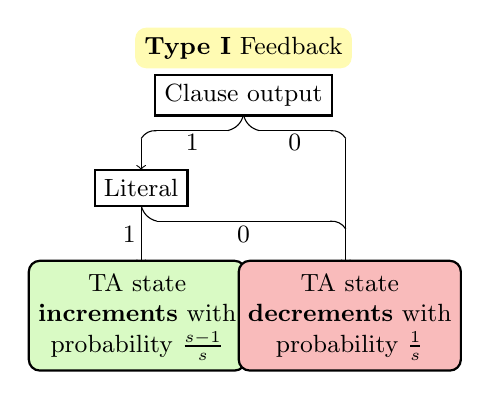
\begin{tikzpicture}[font=\small]
\node [draw=none, shape=rectangle, minimum width=0.8cm, rounded corners, fill=yellow!30!white] at (0,0.6) {\textbf{Type I} Feedback};

\draw []  (0,-0.25) to [bend left] (-0.2,-0.45);
\draw [] (-0.2,-0.45) -- (-1.1,-0.45);
\node[] at (-0.65,-0.6) {1};
\draw []  (-1.1,-0.45) to [bend right] (-1.3,-0.55);
\draw [->] (-1.3,-0.55) -- (-1.3,-0.95);

\draw []  (0,-0.25) to [bend right] (0.2,-0.45);
\draw [] (0.2,-0.45) -- (1.1,-0.45);
\node[] at (0.65,-0.6) {0};
\draw []  (1.1,-0.45) to [bend left] (1.3,-0.55);
\draw [->] (1.3,-0.55) -- (1.3,-2.15);
\node [draw, thick, shape=rectangle, minimum width=0.8cm, fill=white] at (0,0) {Clause output};

\node [draw, thick, shape=rectangle, minimum width=0.8cm] at (-1.3,-1.18) {Literal};
\draw[->] (-1.3,-1.4) -- (-1.3,-2.15);
\node[] at (-1.45,-1.775) {1};
\draw[] (-1.3,-1.4) to [bend right] (-1.1,-1.6);
\draw[] (-1.1,-1.6) -- (1.1,-1.6);
\draw[] (1.1,-1.6) to [bend left] (1.3,-1.7);
\node[] at (0,-1.775) {0};

\node [draw, thick, shape=rectangle, minimum width=0.8cm, rounded corners, fill=new_green] at (-1.35,-2.8) {\begin{tabular}[c]{@{}c@{}} TA state \\ \textbf{increments} with \\ probability $\frac{s-1}{s}$ \end{tabular}};

\node [draw, thick, shape=rectangle, minimum width=0.8cm, rounded corners, fill=new_red!50!white] at (1.35,-2.8) {\begin{tabular}[c]{@{}c@{}} TA state \\ \textbf{decrements} with \\ probability $\frac{1}{s}$ \end{tabular}};

\end{tikzpicture}
}
\hspace{0.2cm}
\subfloat[]{
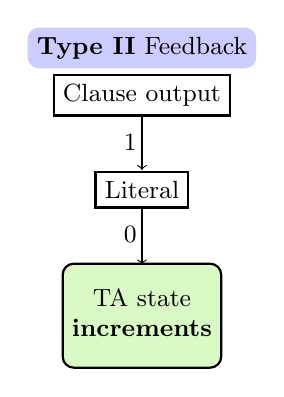
\begin{tikzpicture}[font=\small]
\node [draw=none, shape=rectangle, minimum width=0.8cm, rounded corners, fill=blue!20!white] at (0,0.6) {\textbf{Type II} Feedback};

\draw [->]  (0,-1.4) -- (0,-2.15);
\node[] at (-0.15,-1.775) {0};
\node [draw, thick, shape=rectangle, minimum width=0.8cm, fill=white] at (0,0) {Clause output};
	
\draw [->]  (0,-0.25) -- (0,-0.95);
\node[] at (-0.15,-0.6) {1};
\node [draw, thick, shape=rectangle, minimum width=0.8cm,fill=white] at (0,-1.2) {Literal};

\node [draw, thick, shape=rectangle, minimum width=2cm, minimum height=1.32cm, rounded corners, fill=new_green] at (0,-2.8) {\begin{tabular}[c]{@{}c@{}} TA state \\ \textbf{increments} \end{tabular}};
	
\end{tikzpicture}
}
\vspace{-0.2cm}
\caption{(a) Type I and (b) Type II feedback, where TA state remains unchanged for any other cases.}
\label{fig:type_i_ii}

\Description[Type I/II feedback]

\end{figure}
